\documentclass[10pt]{beamer}
\usetheme{Warsaw}
\usepackage[utf8]{inputenc}
\usepackage[english]{babel}
\usepackage{amsmath}
\usepackage{amsfonts}
\usepackage{amssymb}
\usepackage{graphicx}
\setbeamersize{text margin left=0.3cm,text margin right=0.3cm} 

\renewcommand{\footnotesize}{\scriptsize}

\graphicspath{ {../figures/} }

\usepackage[style=authortitle,doi=false,isbn=false,url=false,backend=bibtex]{biblatex}
\addbibresource{../bvitali_biblio}

%%%%NO_IDEA-BUT_IMPORTANT%%%%
\usepackage{sansmathaccent}
\pdfmapfile{+sansmathaccent.map}
%%%%%%%%%%%%%%%%%%%%%%%%%%%%%

\author[Bastiano Vitali]{{\Large Bastiano Vitali}\\\ \\{\small Prof. Simone Donati (INFN, UniPi)\\ Dr. Pavel Murat (FNAL)}}
\title{In situ monitoring of the stopped muon flux at Mu2e}
%\setbeamercovered{transparent} 
%\setbeamertemplate{navigation symbols}{} 
\titlegraphic{
\includegraphics[scale=0.7]{cherubino.jpg}\ \ 
\includegraphics[scale=0.065]{mu2e_logo}}%%\institute{} 
\date{} 
%\subject{} 

\makeatother
\setbeamertemplate{footline}
{
  \leavevmode%
  \hbox{%
  \begin{beamercolorbox}[wd=.4\paperwidth,ht=2.25ex,dp=1ex,center]{author in head/foot}%
    \usebeamerfont{author in head/foot}\insertshortauthor
  \end{beamercolorbox}%
  \begin{beamercolorbox}[wd=.6\paperwidth,ht=2.25ex,dp=1ex,center]{title in head/foot}%
    \usebeamerfont{title in head/foot}\insertshorttitle\hspace*{3em}
    \insertframenumber{} / \inserttotalframenumber\hspace*{1ex}
  \end{beamercolorbox}}%
  \vskip0pt%
}
\makeatletter
\setbeamertemplate{navigation symbols}{}


\begin{document}

%1
\begin{frame}
\titlepage
\end{frame}

%2
\begin{frame}{Charged Lepton Flavor Violation}
\vspace{0.3cm}
\begin{itemize}
\setlength\itemsep{0.3cm}
\item Lepton Flavor was assumed conserved in the Standard Model (SM)
\item After the discovery of $\nu$ oscillations\footcite{oscillations}, CLFV became a possibility
\item SM + $\nu$ oscillations yield extremely low rates at $\mathcal{O}(10^{-52})$ %\footcite{Signorelli}
\item Many theories enhance the rate: experimental feedback is needed
\end{itemize}
\vspace{0.5cm}
\begin{center}
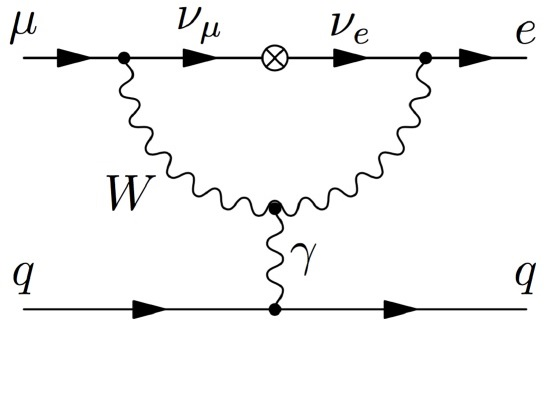
\includegraphics[width=0.4\textwidth]{feynman_mu2e}
\end{center}
\end{frame}

%3
\begin{frame}{History of $\mu\rightarrow e$ searches}
\begin{itemize}
\item Many experiments looking for CLFV (especially using muons)
\end{itemize}
\begin{center}
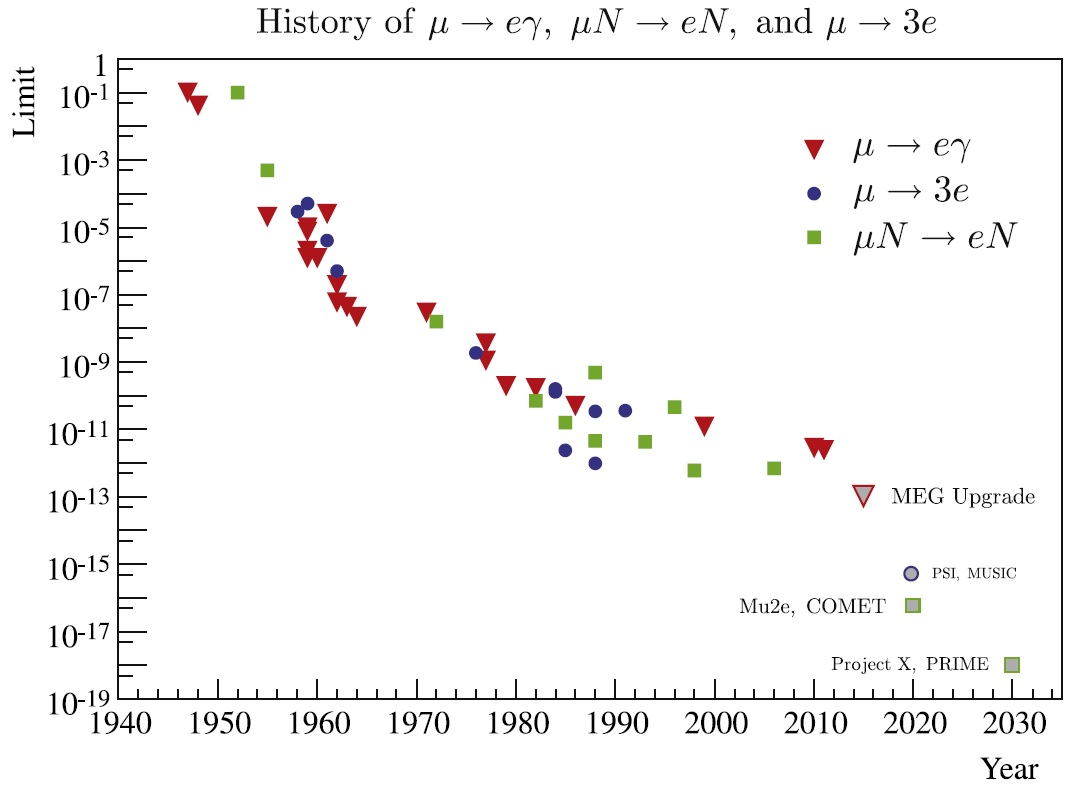
\includegraphics[width=0.8\textwidth]{timeline_measures_2}
\end{center}
\end{frame}

%4
\begin{frame}{Mu2e}
\begin{itemize}
\setlength\itemsep{0.4cm}
\item Mu2e looks for the $\mu^- N \rightarrow e^- N$ process in Al\\
{\small muon to electron conversion in nucleus field}
\item SINDRUM II set the current limit in Au at $7\times10^{-13}$ (90\% C.L.) \footcite{SINDRUMII}
\item The aim is an improvement of 4 order of magnitude
\end{itemize}
\vspace{0.5cm}
\begin{center}
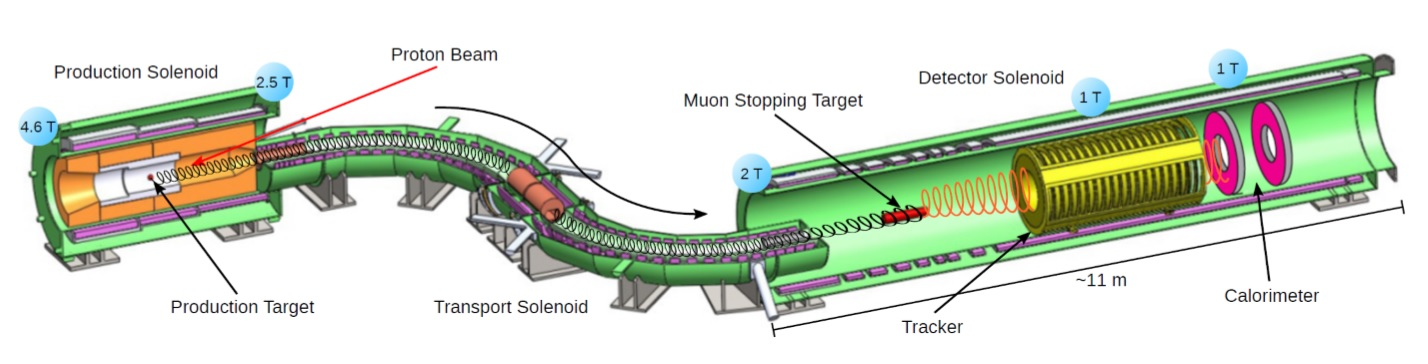
\includegraphics[width=0.9\textwidth]{mu2e_apparatus}
\end{center}
\end{frame}

\begin{frame}
\begin{itemize}
\item Monoenergetic signal: $E_{CE} = m_\mu -B(Z) -E_R(A) \approx 104.97$ MeV
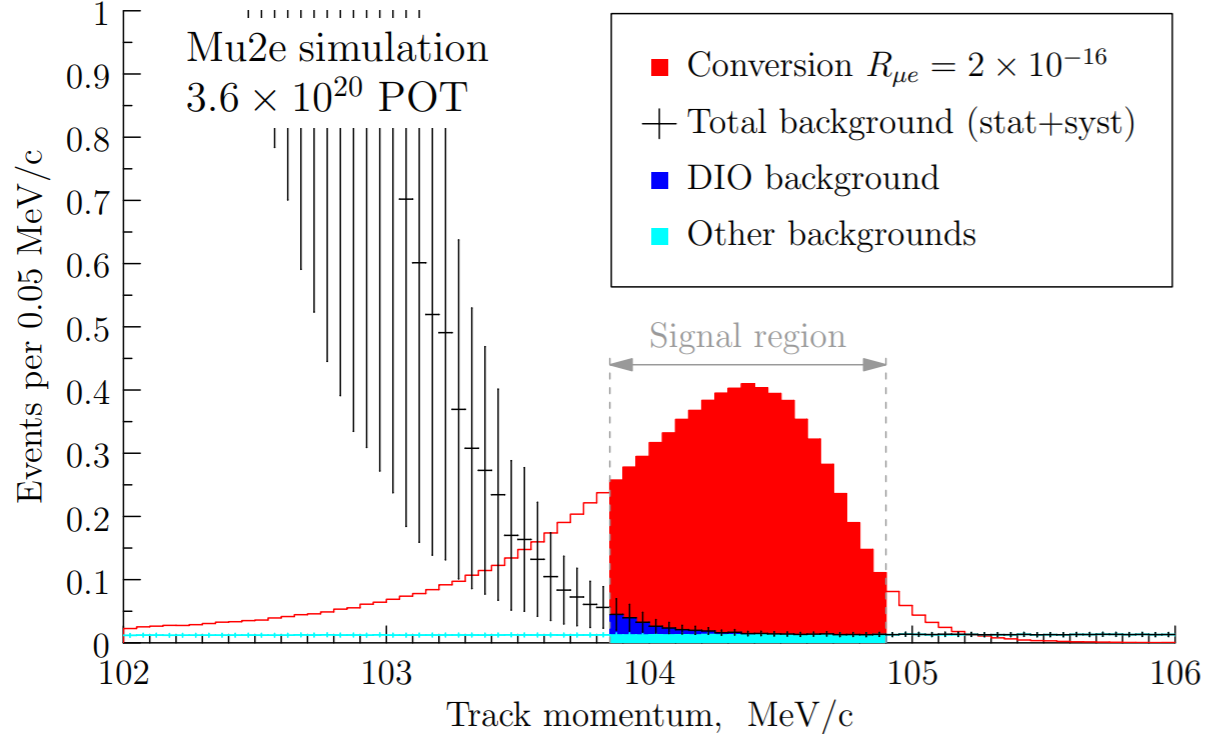
\includegraphics[width=0.8\textwidth]{signal_bg}
\item Background:
\begin{itemize}
\item Muon Decay In Orbit $\rightarrow$ good momentum resolution needed
\item Cosmic rays $\rightarrow$ veto system enclosing the detector
\item Antiproton $\rightarrow$ absorbers in the muon beamline
\item Radiative $\pi$ capture $\rightarrow$ pulsed beam + beam extinction
\end{itemize}
\end{itemize}
\end{frame}

%
\begin{frame}{Straw-tube tracker}
\centering
\begin{itemize}
\item 18 stations of straw tubes creating a hollow cylinder
\end{itemize}
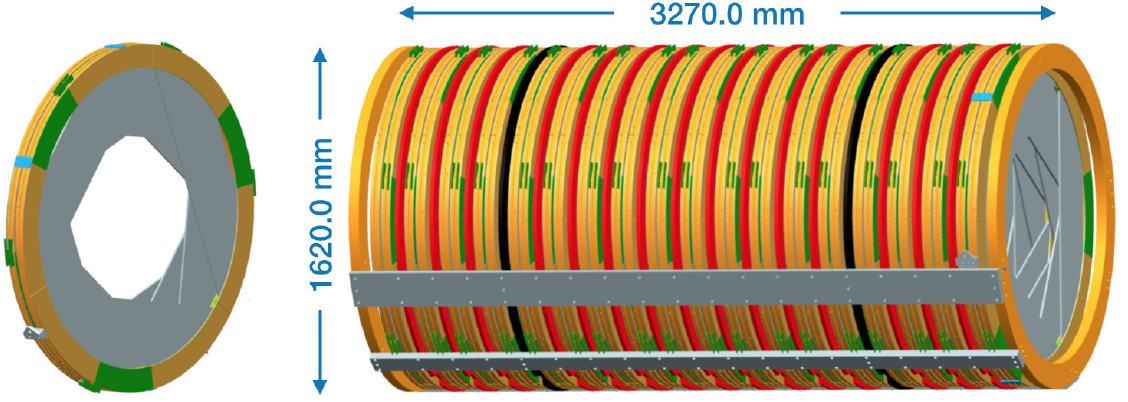
\includegraphics[width=0.8\textwidth]{Tracker_2}
\begin{itemize}
\item The radii define the momentum acceptance
\end{itemize}
\vspace{0.2cm}
\resizebox{.8\textwidth}{!}{
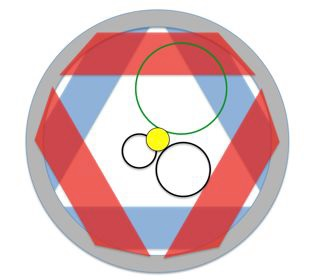
\includegraphics[height=2.5cm]{mu2e_tracker_front}
\quad
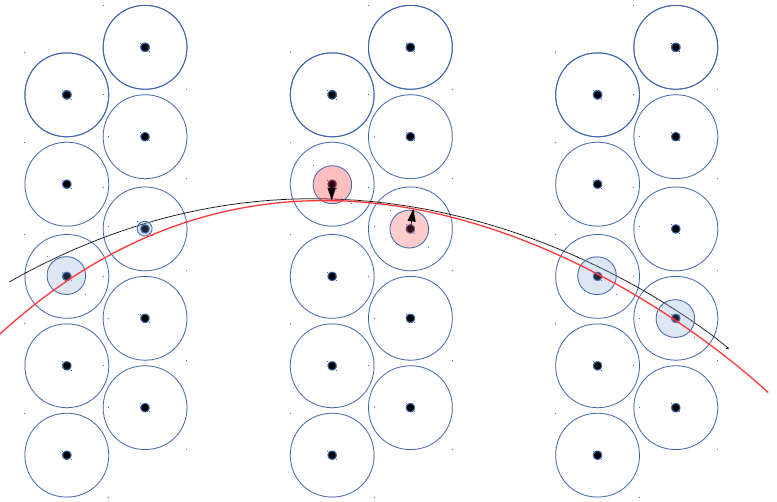
\includegraphics[height=2.5cm]{ambiguity}
}
\end{frame}

%
\begin{frame}{Calorimeter}
\begin{itemize}
\item Two disks (70 cm apart) of CsI crystals
\item Crystals are read by SiPMs (two for redondance)
\end{itemize}
\centering
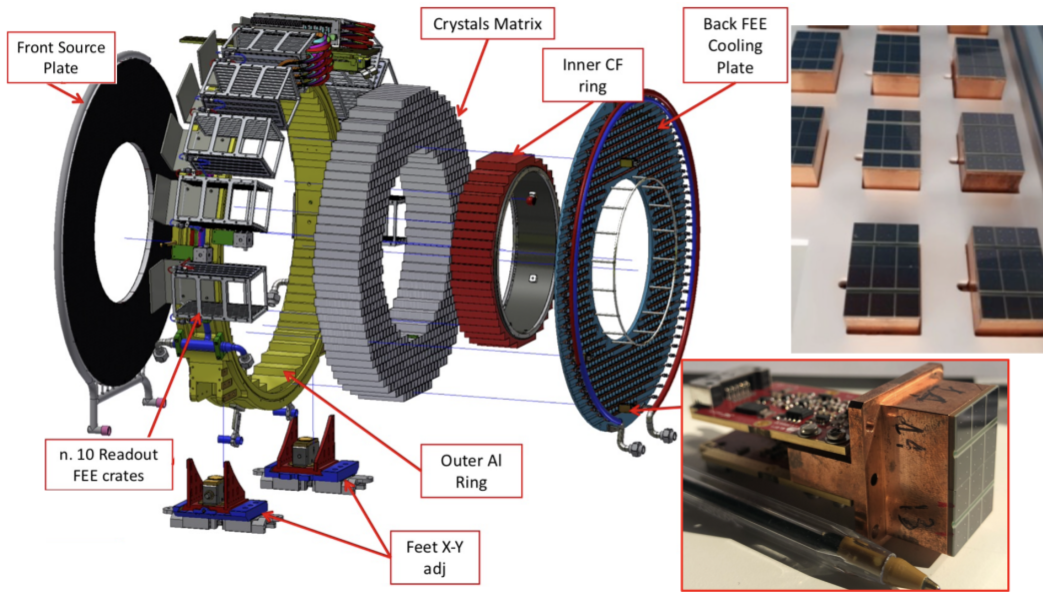
\includegraphics[width=0.8\textwidth]{mu2e_calorimeter_disk_2}
\end{frame}


%
\begin{frame}{Mu2e: Time structure}
\centering
\begin{itemize}
\item A proton pulsed beam to reduce background from $\pi$
\end{itemize}
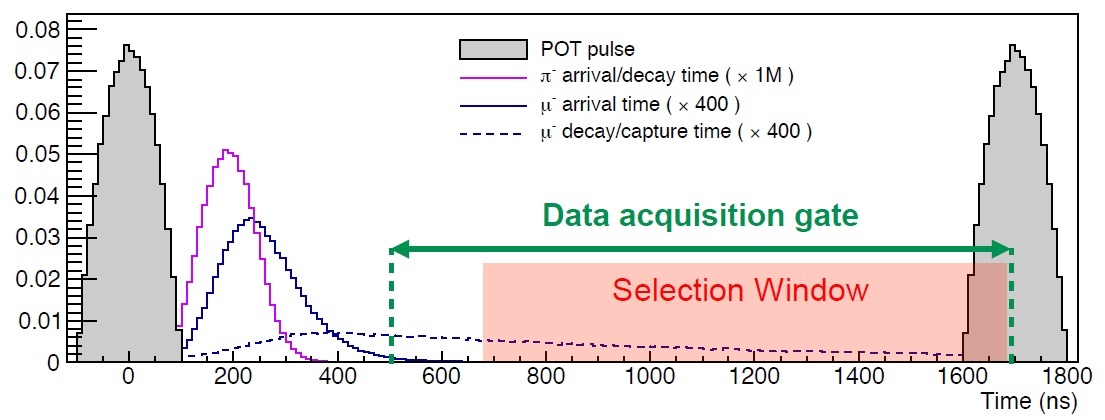
\includegraphics[width=0.8\textwidth]{mu2e_event}
\begin{itemize}
\item Pulses (grouped in \textit{spills}) obtained through \textit{resonant extraction}
\end{itemize}
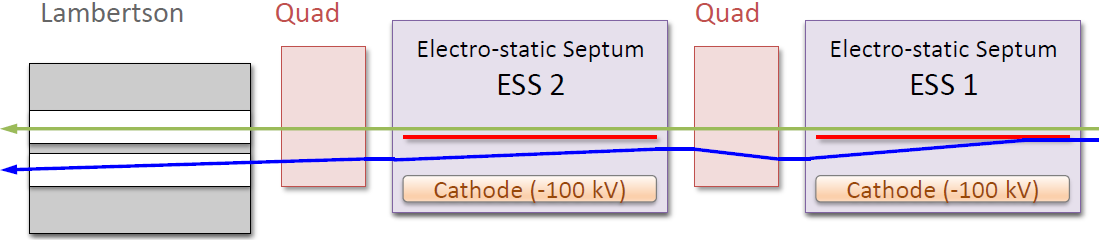
\includegraphics[width=0.8\textwidth]{Extraction}
\end{frame}

%
\begin{frame}{Spill simulation}
\begin{itemize}
\item Resonant extraction $\rightarrow$ beam intensity variations on ms time-scale \footcite{SpillSim}\\
\end{itemize}
\begin{center}
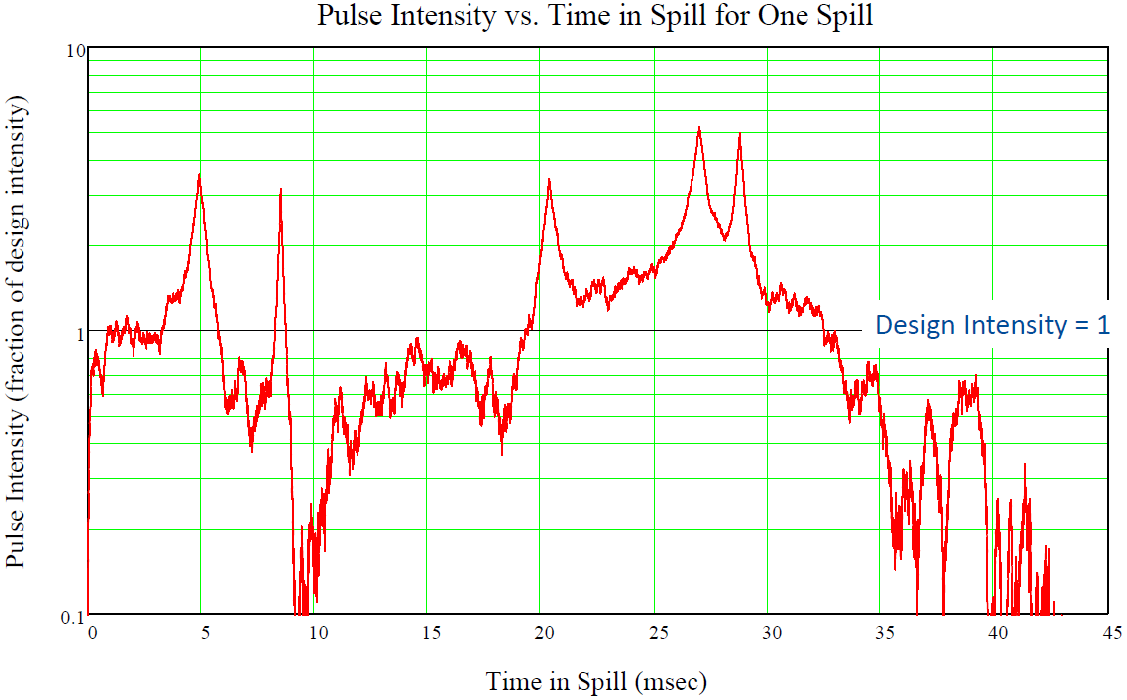
\includegraphics[width=0.8\textwidth]{POT_sim}
\end{center}
\end{frame}

\begin{frame}{Why is important?}
\begin{itemize}
\item The reconstruction efficiency changes \footcite{MDC2018:PBI} and so does the CRV response \footcite{MDC2018}
\end{itemize}
\begin{center}
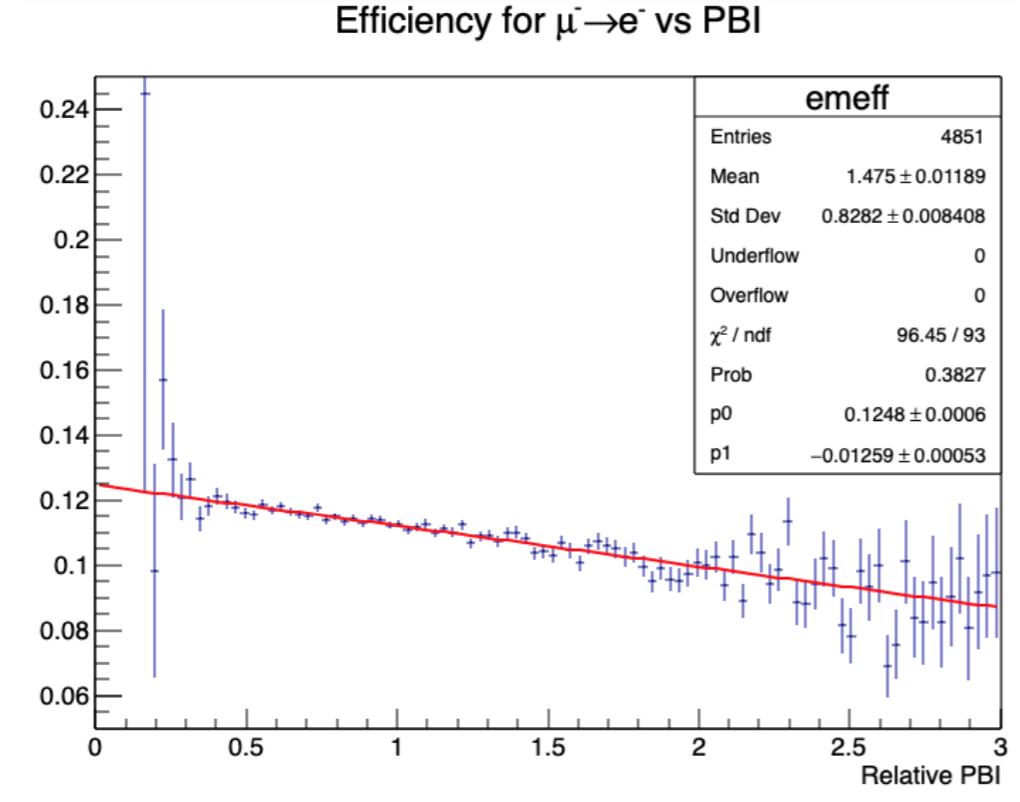
\includegraphics[width=0.6\textwidth]{Dave_eff-vs-PBI}
\end{center}
\end{frame}

%
\begin{frame}{Monitor these fluctuations}
Time-scale of ms $\rightarrow$ Physical processes as handles?
\vspace{0.3cm}
\begin{itemize}
\setlength\itemsep{0.5cm}
%\pause %%%
\item Photons from stopped muons $\rightarrow$ HPGe and LaBr$_3$(Ce) \footcite{STM:2016} \footcite{LaBr3:2020}\\
\begin{itemize}
\setlength\itemsep{0.2cm}
\item Optimal for the overall normalization\\
\item LaBr$_3$ $\rightarrow$ measurement at $10\%$ on $2\div3$ \textit{supercycles} ($\approx 3.5$ s) \footcite{LaBr3:2019}
\end{itemize}
%\pause %%%
\item Nuclear muon capture $\rightarrow$ ejected proton counting
\begin{itemize}
\setlength\itemsep{0.2cm}
\item NPOT $\times$ $\mu_{stop}$/POT $\times$ capt/$\mu_{stop}$ $\times$ p/capt $\sim 2\times10^3$ p/$1.7\ \mu$s\\
\item Low $\beta$: high energy deposition ($\sim 1/\beta^2$) and multiple scattering ($\sim 1/\beta p$)
\item Absorber impacts the momentum
\end{itemize}
\end{itemize}
\end{frame}

%
\begin{frame}{Track fitting: Hits and clustering}
\begin{itemize}
\item Tracker
\begin{itemize}
\item Straws are read by both ends: $\Delta t \rightarrow$ position along the wire
\item Hits grouped in Time Clusters (checking also the XY position)
\end{itemize}
\item Calorimeter
\begin{itemize}
\item Crystal signals are grouped in Clusters
\item Clusters in the calorimeter can be used to seed the algorithm
\end{itemize}
\end{itemize}
\centering
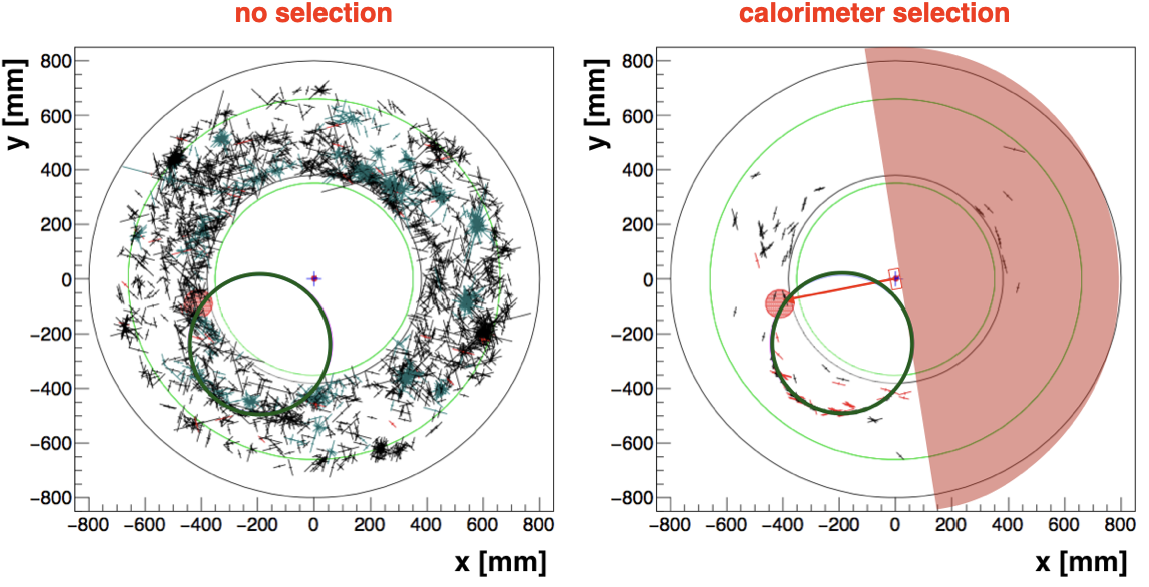
\includegraphics[width=0.8\textwidth]{giani_CalPatRec_semiplane}
\end{frame}

%
\begin{frame}{Track fitting: Pattern recognition}
\noindent
\begin{minipage}{.6\textwidth}
	\begin{itemize}
	\item Triplets in XY to find the center
	\begin{itemize}
	\setlength\itemsep{0.2cm}
		\item Intersect the perpendicular bisectors
		\item Loop to find the radius
	\end{itemize}
	\end{itemize}
\end{minipage}
\begin{minipage}{0.35\textwidth}
    \centering
    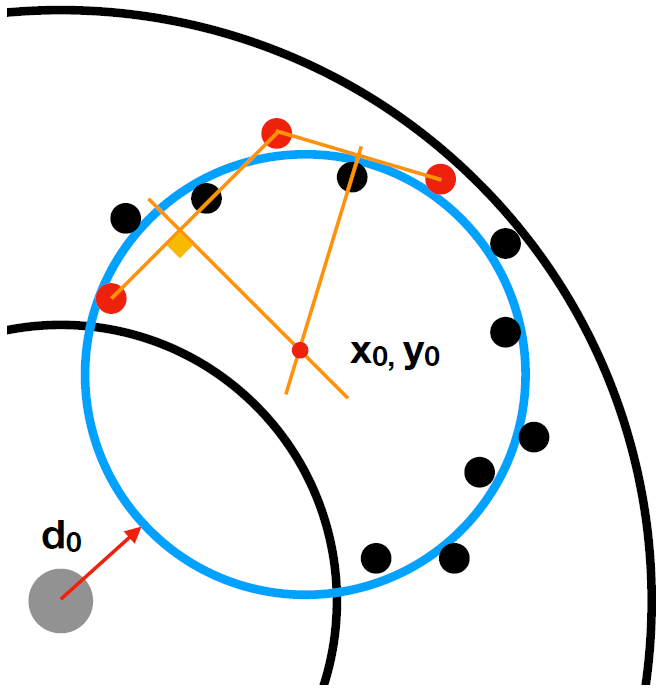
\includegraphics[width=0.7\textwidth]{giani_TrkPatRec_triplets}
\end{minipage}

\begin{itemize}
\item In $\Phi$Z, after solving the `2$\pi$-ambiguity', is linear fit 
	\begin{itemize}
	\setlength\itemsep{0.2cm}
		\item Estimate of $\lambda$ needed
		\item Found using couples of hits
	\end{itemize}
\end{itemize}
\centering
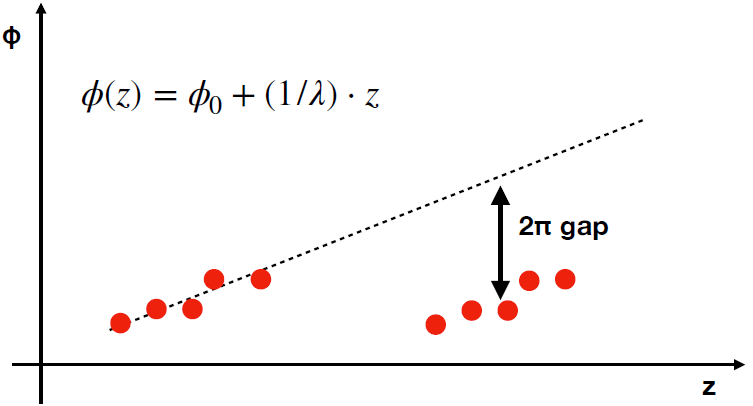
\includegraphics[width=0.4\textwidth]{giani_TrkPatRec_ambiguity0}
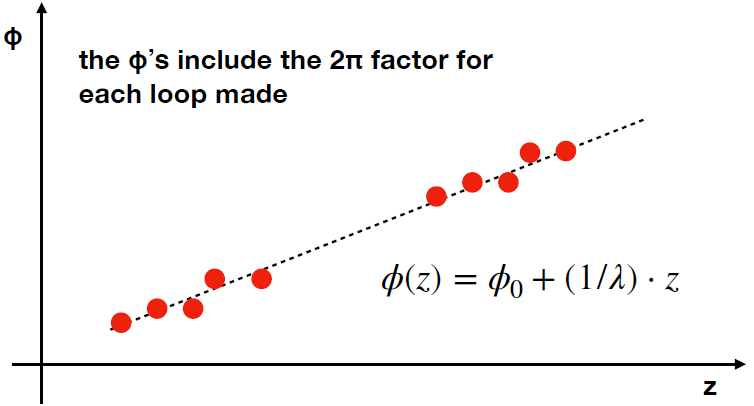
\includegraphics[width=0.4\textwidth]{giani_TrkPatRec_ambiguity1}
\end{frame}

%
\begin{frame}{Track fitting: Kalman filter}

\noindent
\begin{minipage}{.6\textwidth}
	\begin{itemize}
	\setlength\itemsep{0.4cm}
	\item Track of 5 parameters ${\vec{\eta}} \equiv ( d_0, \phi_0, \omega, z_0, \tan \lambda)$
	\item Non uniform field, energy loss, scattering \\${\vec{\eta}}$ can depend on the position 
	\item Kalman filter: 
	\begin{itemize}
	\setlength\itemsep{0.2cm}
	\item Iteratively `add hits' to the track
	\item Easy to implement and fast (5x5 matrices)
	\item Allows best estimate in any point
	\end{itemize}
	\end{itemize}
\end{minipage}
\begin{minipage}{0.35\textwidth}
    \centering
	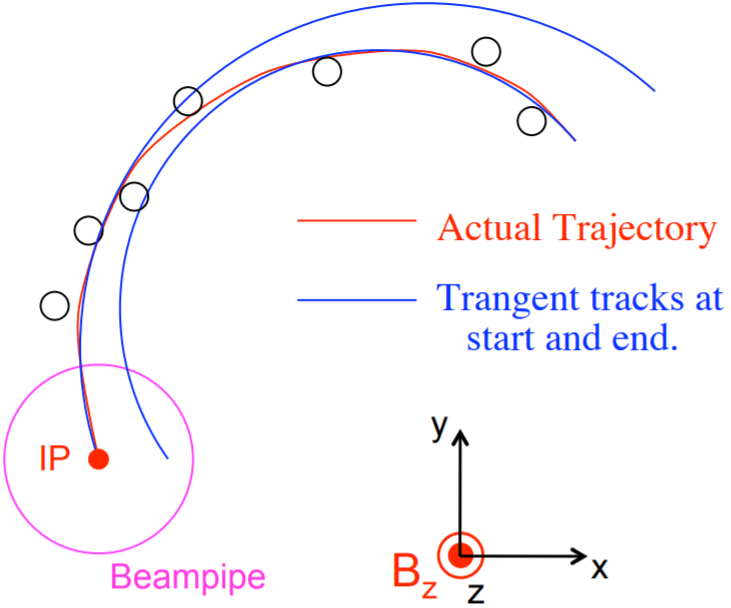
\includegraphics[width=1\textwidth]{Kutschke_Kalman_circ}
\end{minipage}
\end{frame}

%
\begin{frame}{Flat single protons}
\begin{itemize}
\item 100k protons generated with flat momentum [100,600] MeV/c
\end{itemize}
\begin{center}
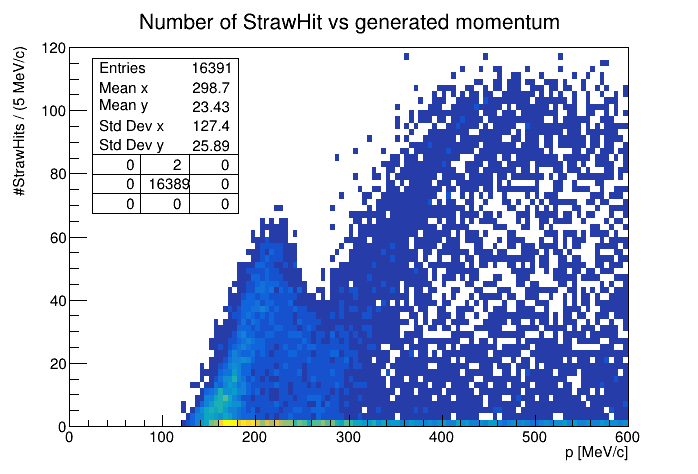
\includegraphics[width=0.8\textwidth]{plots/flat/all_SHvsGenp}
\end{center}
\end{frame}

%
\begin{frame}{Flat single protons: What is the dip?}
\begin{itemize}
\item Let's see where the trajectories start and end
\end{itemize}
\begin{center}
\only<1>{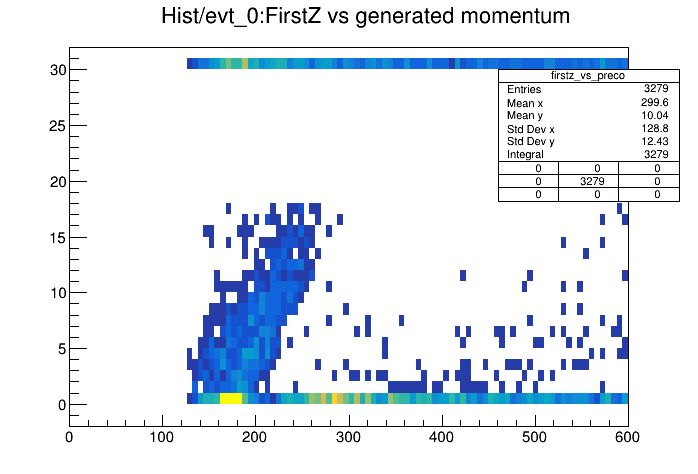
\includegraphics[width=0.8\textwidth]{/plots/flat/Lambda_first-z}}
\only<2>{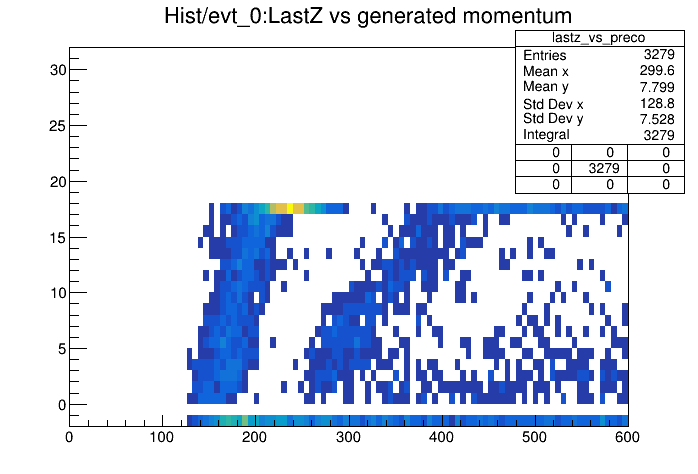
\includegraphics[width=0.8\textwidth]{/plots/flat/Lambda_last-z}}
\end{center}
\end{frame}

%
\begin{frame}{Flat single protons: What is the dip?}
\begin{itemize}
\item The tracker is finite: Topology changes at $\sim 250$ MeV/c
\end{itemize}
\begin{center}
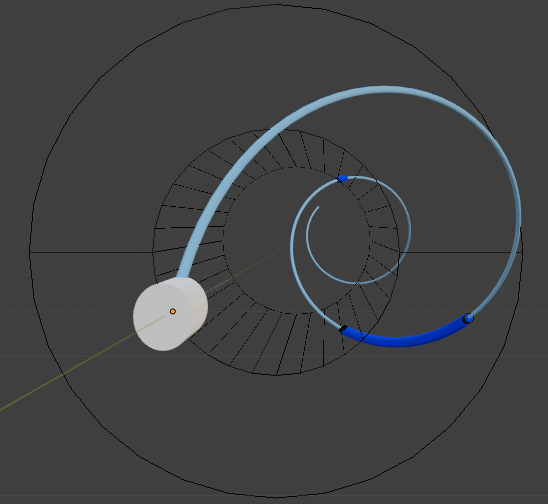
\includegraphics[scale=0.7]{Blender_Tracker_4}
\end{center}
\end{frame}

%
\begin{frame}{Flat single protons: Algorithm efficiency}
\begin{itemize}
\item The reconstruction seems to be working
\end{itemize}
\begin{center}
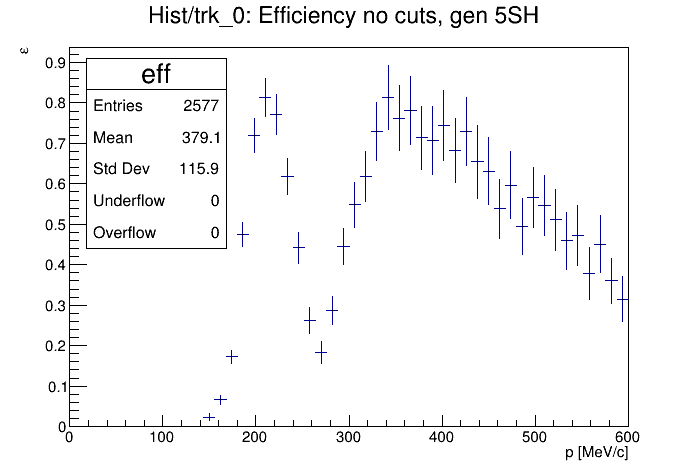
\includegraphics[width=0.8\textwidth]{plots/flat/Lambda_eff_trk0-5hits}
\end{center}
\end{frame}

%
\begin{frame}{Flat single protons: Time Clusters}
\begin{itemize}
\item Side note: some events with more than 1 Time Cluster
\end{itemize}
\begin{center}
\only<1>{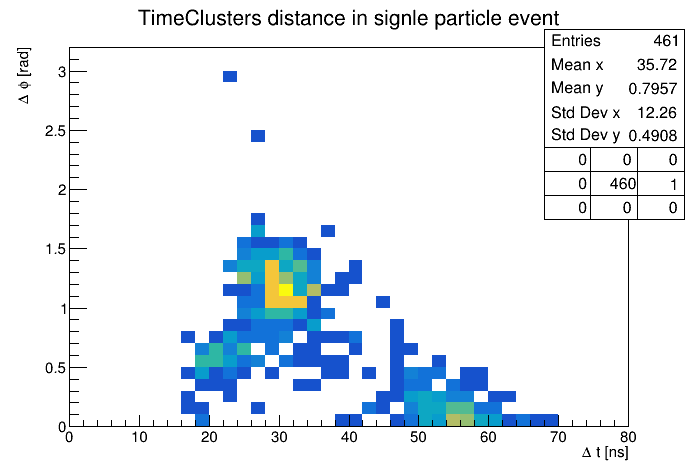
\includegraphics[width=0.8\textwidth]{plots/flat/TimeClusterPar_ProtonPeaks}}
\only<2>{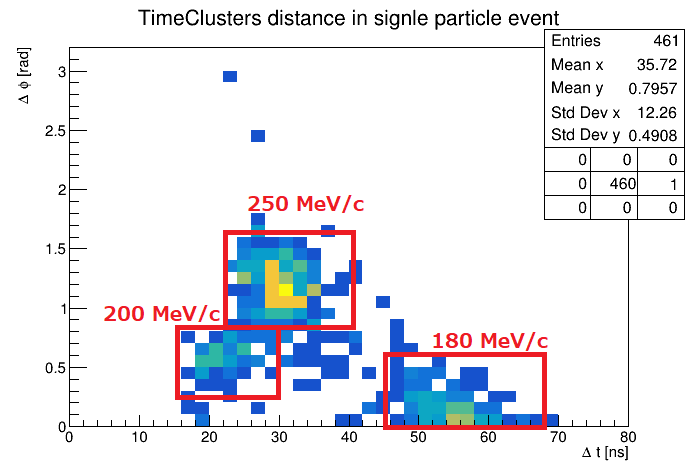
\includegraphics[width=0.8\textwidth]{plots/flat/TimeClusterPar_ProtonPeaks_boxes}}
\end{center}
\end{frame}

%
\begin{frame}{Flat single protons: Topology}
\begin{itemize}
\item Reconstructable high momentum particles are emitted forward
\item Could be useful for tracker alignment
\end{itemize}
\begin{center}
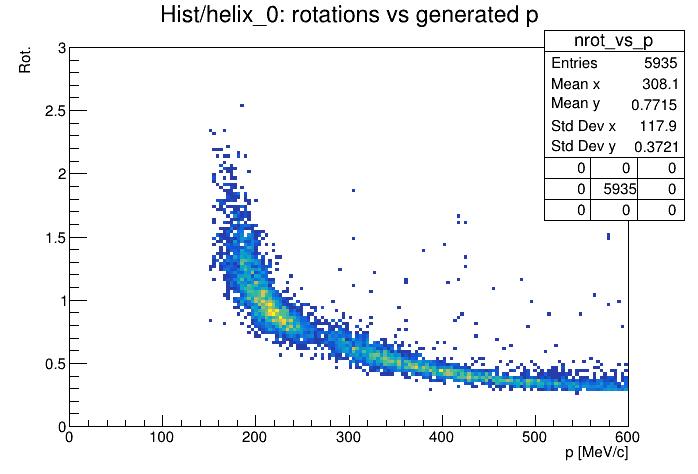
\includegraphics[width=0.8\textwidth]{plots/flat/Lambda_Rot-vs-p}
\end{center}
\end{frame}

%
\begin{frame}{Flat single protons: Momentum reconstruction}
\begin{itemize}
\item Good reconstructed momentum; we see the effect of the absorbers
\end{itemize}
\begin{center}
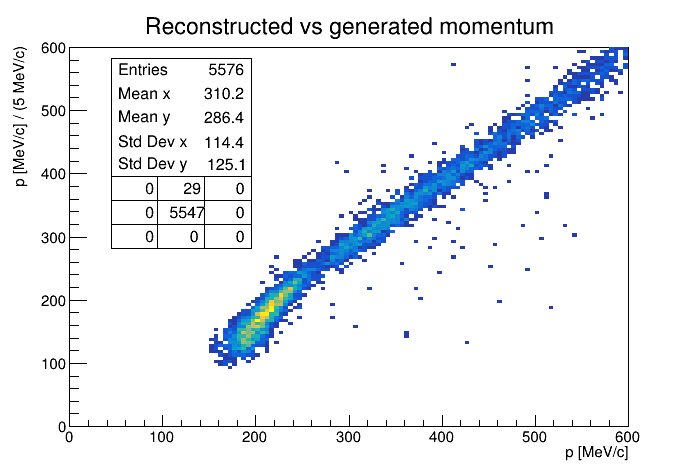
\includegraphics[width=0.8\textwidth]{plots/flat/Lambda_preco-vs-pgen}
\end{center}
\end{frame}

%
\begin{frame}{Ejection spectra}
\begin{itemize}
\item Parameterization by Murat \footcite{Pasha:spectra} after TWIST \footcite{TWIST:2020} and AlCap \footcite{AlCap:2020} results\\
{\small Followed a comparison to Hungerford parameterization and discussion \footcite{io:sobottka}}
\end{itemize}

\begin{center}
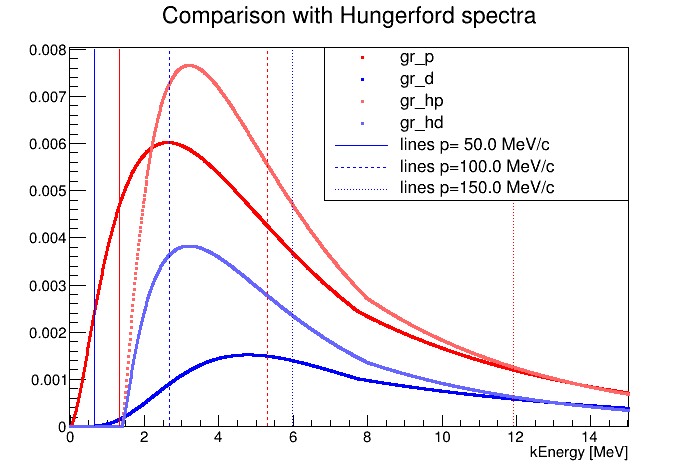
\includegraphics[width=0.65\textwidth]{mu2e_spectra_articles/comparison2}
\end{center}
\end{frame}

%
\begin{frame}{Single protons: Efficiency}
\begin{itemize}
\item Protons generated with the expected spectra: Hungerford in red
\item Compatible number of reconstructed: $\approx 2.7$ \textperthousand
\end{itemize}
\begin{center}
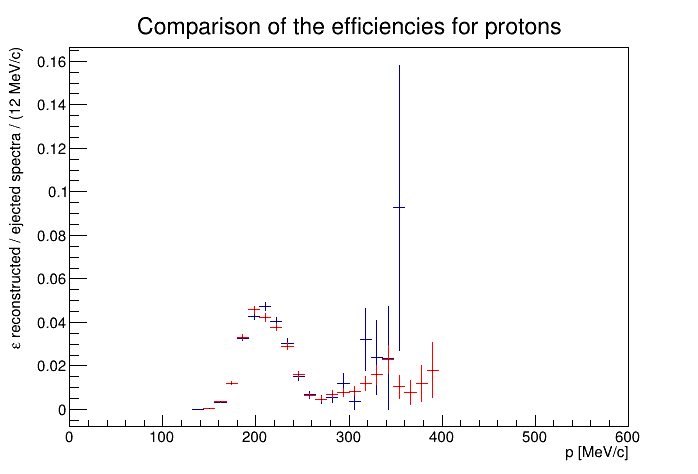
\includegraphics[width=0.8\textwidth]{plots/ejected/proton_eff_comparison}
\end{center}
\end{frame}

%
\begin{frame}{Single deuterons: Efficiency}
\begin{itemize}
\item Deuterons generated with the expected spectra: Hungerford in red\\
\item Number of reconstructed increases: $\approx 0.5\rightarrow 1$ \textperthousand
\end{itemize}
\begin{center}
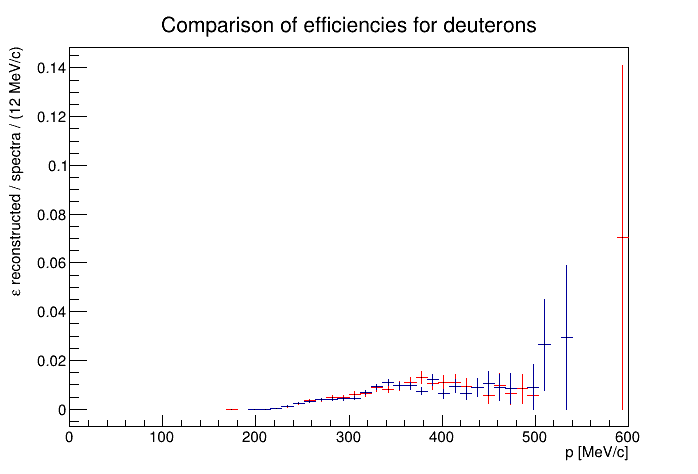
\includegraphics[width=0.8\textwidth]{plots/ejected/deuterons_eff_comparison}
\end{center}
\end{frame}

%
\begin{frame}{Mixed events: Charge cut}
\begin{itemize}
\item How can we isolate proton hits?
\end{itemize}
\begin{center}
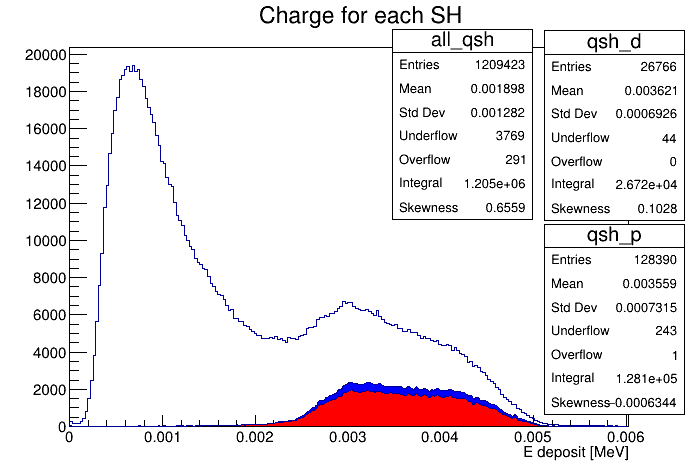
\includegraphics[width=0.8\textwidth]{plots/mix/mix500_qsh_Ps}
\end{center}
\end{frame}

%
\begin{frame}{Mixed events: Charge cut}
\begin{itemize}
\item With a cut at 2 keV the reconstruction improves
\end{itemize}
\begin{center}
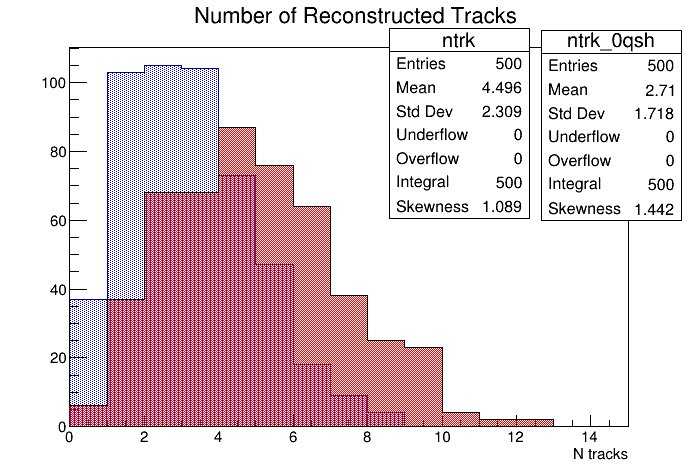
\includegraphics[width=0.8\textwidth]{plots/mix/mix500_trk_Ps}
\end{center}
\end{frame}

\begin{frame}{Mixed events: Quality}
\begin{itemize}
\item How many `fake' tracks do we reconstruct? 
\end{itemize}
\centering
%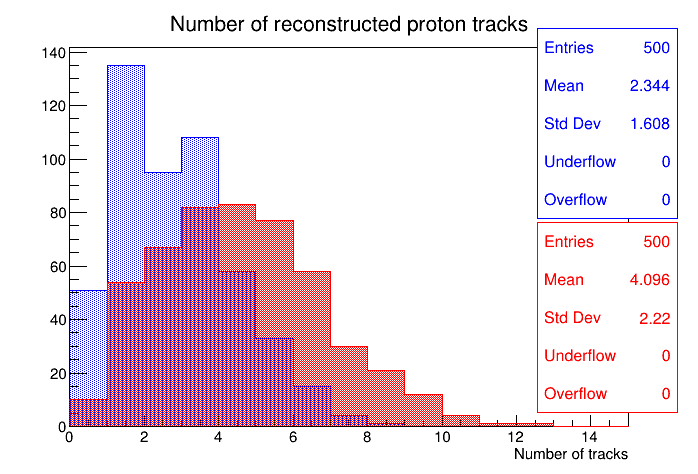
\includegraphics[width=0.8\textwidth]{/plots/mix/mix500_trk_p}
%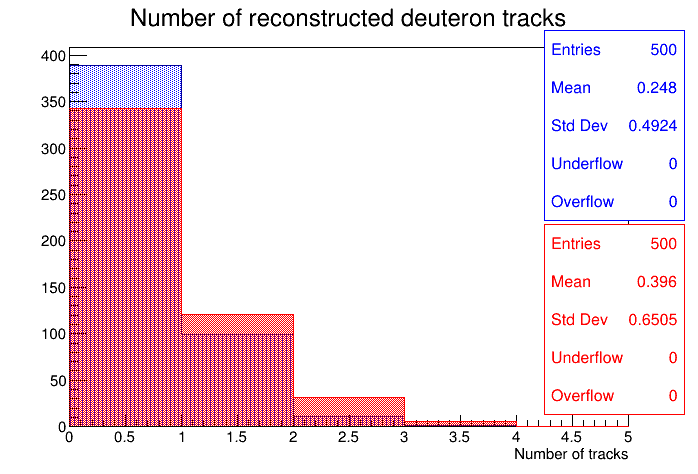
\includegraphics[width=0.8\textwidth]{/plots/mix/mix500_trk_d}
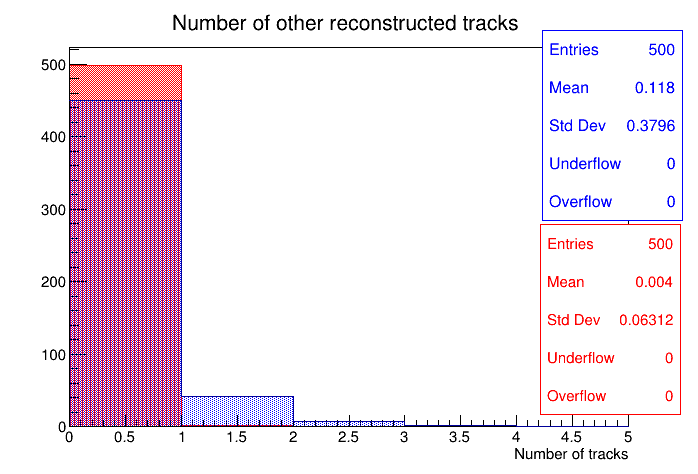
\includegraphics[width=0.8\textwidth]{/plots/mix/mix500_trk_o}
\end{frame}

%
\begin{frame}{Beam intensity}
\begin{itemize}
\item How does the number of tracks depend on the beam intensity?
\end{itemize}
\begin{center}
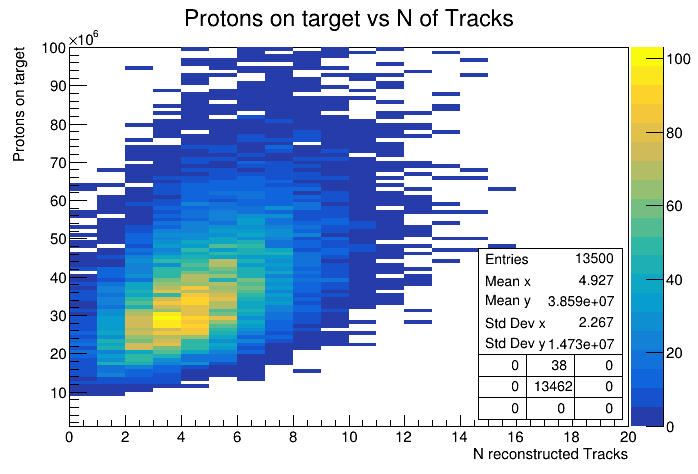
\includegraphics[width=0.8\textwidth]{plots/mix/lum_vs_ntrk}
\end{center}
\end{frame}

%
\begin{frame}{Mixed events: Beam intensity}
\begin{itemize}
\item Slicing assuming 10\% variation in 1 ms
\end{itemize}
\begin{center}
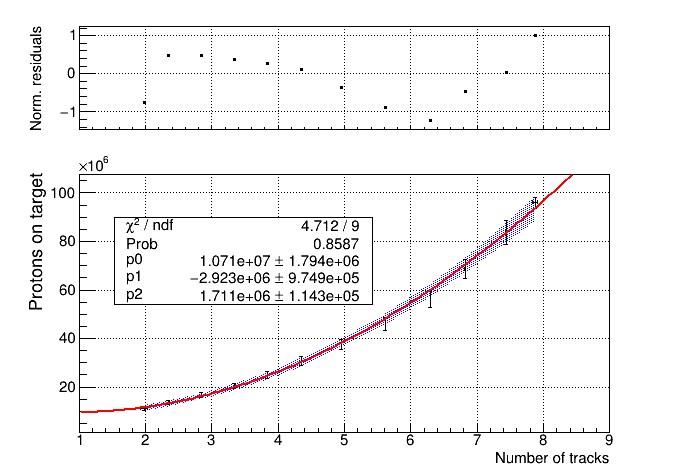
\includegraphics[width=0.8\textwidth]{plots/mix/pol2-fit}
\end{center}
\end{frame}

%
\begin{frame}{Mixed events: Uncertainty}
\begin{itemize}
\item Assume $<$n$>$ tracks in 1 ms $\rightarrow$ Relative uncertainty on the PBI? (first look)
\end{itemize}
\begin{center}
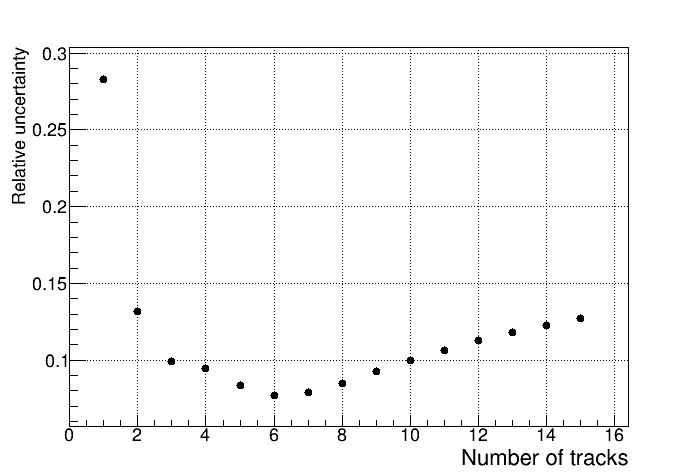
\includegraphics[width=0.8\textwidth]{plots/mix/uncertainty}
\end{center}
\end{frame}

%
\begin{frame}{Conclusion}
\begin{itemize}
\setlength\itemsep{0.4cm}
\item We successfully reconstruct these particles
\item A monitor on the ms timescale seems feasible ($\lesssim 15 \%$) 
\item Some improvement in the time clustering procedure
\item Update with new code, spectra and mixing ratio
\end{itemize}
\vspace{1cm}
\centering
{\large \textbf{Thanks for your attention!}}
\end{frame}

%REF
%\setbeamertemplate{bibliography item}{}
\begin{frame}[allowframebreaks]{References}
\printbibliography[heading=none]
\end{frame}


\end{document}
%%%%%%%%%%%%%%%%%%%%%%%%%%%%%%%%%%%%%%%%%%%%%%%%
%%%%%%%%%%%%%%%%%%%%%%%%%%%%%%%%%%%%%%%%%%%%%%%%

%%%%%%%%%%%%%%%%%%%%%%%%%%%%%%%%%%%%%%%%%%%%%%%%
%%%%%%%%%%%%%%%%%%%%%%%%%%%%%%%%%%%%%%%%%%%%%%%%

%%%%%%%%%%%%%%%%%%%%%%%%%%%%%%%%%%%%%%%%%%%%%%%%
%%%%%%%%%%%%%%%%%%%%%%%%%%%%%%%%%%%%%%%%%%%%%%%%
\begin{itemize}
\item After $\nu$ oscillation, Charged Lepton Flavour Violation is an open question
\item Mu2e looks for $\mu\rightarrow e$ conversion (near Al$^{27}$ nucleus)
\begin{itemize}
\item In the SM, depends on $\Delta m_{\nu}^2 \rightarrow$ BR$\approx10^{-54}$
\item Many theories, SUSY among them, predict higher BR
\item The aim is Single Event Sensitivity of $10^{-17}$
\end{itemize}
\begin{figure}
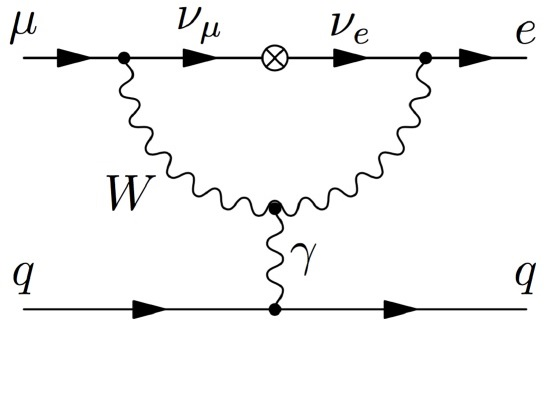
\includegraphics[scale=0.4]{feynman_mu2e}
\caption{SM Feynman diagram of $\mu\rightarrow e$ conversion}
\end{figure}
\end{itemize}

\begin{center}
\resizebox{.9\textwidth}{!}{%
\includegraphics[height=3cm]{example-image-a}%
\quad
\includegraphics[height=3cm]{example-image-16x9}%
}
\end{center}


%%%%%%%%%%%%%%

%%%Devi usre LuaLaTex
\usepackage{tikz-feynman}
\tikzfeynmanset{compat=1.0.0} 
%%%%NO_IDEA-BUT_IMPORTANT%%%%
\usepackage{sansmathaccent}
%\pdfmapfile{+sansmathaccent.map}
%%%%%%%%%%%%%%%%%%%%%%%%%%%%%
\feynmandiagram [horizontal=a to b] {
i1 -- [fermion] a -- [fermion] i2,
a -- [photon] b,
f1 -- [fermion] b -- [fermion] f2,
};

\feynmandiagram [layered layout, horizontal=b to c] {
a -- [photon, momentum=\(p\)] b
-- [fermion, half left, looseness=1.5, momentum=\(k\)] c
-- [fermion, half left, looseness=1.5, momentum=\(k-p\)] b,
c -- [photon, momentum=\(p\)] d,
};